\documentclass{article}
\title{Project 4: Locks and Threads}
\author{JuranDing}
\date{2018-12-07}
\usepackage{amsmath}
\usepackage{graphicx}
\usepackage{listings}
\usepackage{subcaption}
\usepackage{cite}
\usepackage{siunitx}
\usepackage{multirow}
\usepackage{booktabs}
\usepackage{longtable}
\usepackage{tikz}
\usepackage{palatino}
\usepackage{booktabs}
\usepackage[section]{placeins}
\usepackage{float}
\usepackage{geometry}
\graphicspath{{./}}
\usetikzlibrary{shapes.geometric, arrows}
\lstset{
	numberstyle= \tiny,     
	keywordstyle= \color{ blue!70},
	commentstyle=\color{red!50!green!50!blue!50},    
	frame=shadowbox,    
	rulesepcolor= \color{ red!20!green!20!blue!20}  } 

\begin{document}
	\tableofcontents
	\pagenumbering{gobble}
	\maketitle
	\pagenumbering{arabic}
	\section{Wrapper}
	Before I realize a lock, there are some preparations for the lock implementation like atomic operation and futex wrapper.
	\subsection{Atomic Operation}
	The atomic operation is not implemented with pure C language but with assemble language and some inner built system call by the support of x86 architecture. And I list some atomic operations that will be used in the lock-make program. \\
	\begin{itemize}
		\item Assemble Language Operation \\
		
		\begin{itemize}
			\item \textbf{xchg} \\
			In the following code, \emph{asm volatile} means that the sentence in the brackets should be explained as the assemble language. The sentence is generally divided into 4 sectors in the extended Asm. The first is \emph{instruction}, and the second is \emph{output}  operation while the third is \emph{input}. The first 3 sectors are easy to understood. The 4th is called \emph{Clobber List} which is used to inform gcc that we will use and modify some hardware registers ourselves and the value loaded into these registers won't be valid. Like the \emph{cc}, it tells gcc that instruction can alter the condition code register to avoid some unpredictable conditions. And the specific explanation is in the code's annotations.\\
			\begin{lstlisting}
static inline uint
xchg(volatile unsigned int *addr, unsigned int newval)
{
	uint result;
	//lock means that the operation is atomic
	//xchgl means exchange values
	asm volatile("lock; xchgl %0, %1" :
	/*
	 * "+m" "+" is a modifier means that operation 
	 * for the varaible is reading or writing
	 * "m" is memory constrain, the variable should 
	 * be a memory
	 */  
	 
	/*
	 * "=a", "=" means that the variable is write-only
	 * "a" is a kind of register starting with "a"
	 */ 
		"+m" (*addr), "=a" (result) : 
	/*
	 * "1" means that the valuable mathching the number 
	 * in the instruction
	 */
		"1" (newval) : 
	/*
	 *  As the condition codes will be changed, 
	 *  we are adding "cc" to clobberlist.
	*/
		"cc");
	return result;
}
			\end{lstlisting}
		\end{itemize}
		\item Inner-Built Function \\ \\
		The following builtins are intended to be compatible with those described in the Intel Itanium Processor-specific Application Binary Interface. In most cases, these builtins are considered a full barrier. That is, no memory operand will be moved across the operation, either forward or backward. Further, instructions will be issued as necessary to prevent the processor from speculating loads across the operation and from queuing stores after the operation. \\
		\begin{itemize}
			\item \textbf{\_\_sync\_val\_compare\_and\_swap(type *ptr, type oldval type newval)}  \\ \\
			That is, if the current value of *ptr is oldval, then write newval into *ptr. There are some tricks to use the operation which is about return value. When the comparison is successful the value returns one while it returns the content \emph{addr}. So if the original value of addr is 1, no matter the comparison successful or failed, it will return true. The characteristic can be used to reduce code efficiently. \\
			\begin{lstlisting}
\_\_sync\_val\_compare\_and\_swap(type *ptr, 
	type oldval type newval)
{
	if(*ptr == oldval)
	{
		*ptr = newval;
		return 1;
	}
	else return *addr;
}
			\end{lstlisting}
			\item \textbf{\_\_sync\_lock\_test\_and\_set (type *ptr, type value, ...)} \\ \\
			This builtin, as described by Intel, is not a traditional test-and-set operation, but rather an atomic exchange operation. It writes value into *ptr, and returns the previous contents of *ptr. The deference between the \emph{test and set} and the \emph{swap and compare} is that the latter doesn't need a compare, just set the value to the \emph{addr}. Here's the programming logic with pseudocode:
			\begin{lstlisting}
__sync_lock_test_and_set (type *ptr, type value, ...)
{
	tmp  = *ptr;
	*ptr = value;
	return tmp;
}
			\end{lstlisting}
			\item \textbf{\_\_sync\_fetch\_and\_add} \\ \\
			It's used to implement a atomic \emph{++}. It begins fetch before the specific arithmetic operations or the logic operation. Some other arithmetic operations or the logic operations are applied to it too. Here's the programming logic with pseudocode:
			\begin{lstlisting}
\_\_sync\_fetch\_and\_add(type *addr, type value)
{
	tmp = *addr ;
	*addr += value;
	return tmp;
}
			\end{lstlisting}
			\item \textbf{\_\_sync\_sub\_and\_fetch} \\ \\
			It's used to implement a atomic  \emph{- -}. It begins the specific arithmetic operations or the logic operation before fetch. Some other arithmetic operations or the logic operations are applied to it too. Here's the programming logic with pseudocode:
			\begin{lstlisting}
\_\_sync\_fetch\_and\_add(type *addr, type value)
{
	tmp = *addr -value ;
	*addr -=  value;
	return tmp;
}
			\end{lstlisting}
		\end{itemize}
	\end{itemize} 
	\subsection{Futex Wrapper}
	To implement the mutex, we need to stop the thread for a while (let it sleep), and the linux system provides us the function to sleep the thread called futex. The parameters passing is trivial so we need a wrapper. \\
	\subsubsection{Futex}
	Just paste the code:
	\begin{lstlisting}
int futex(int *uaddr, int futex_op, int val, 
	const struct timespec *timeout, int *uaddr2, int val3)
{
	return syscall(SYS_futex, uaddr, 
		futex_op, val,timeout, uaddr, val3);
}
	\end{lstlisting}
	\subsubsection{Futex\_Wait}
	This operation tests that the value at the futex word pointed to by the address uaddr still contains the expected value val, and if so, then sleeps waiting for a FUTEX\_WAKE operation on the futex word. The purpose of the comparison with the expected value is to prevent lost wake-ups. \\
	\begin{lstlisting}
void futex_wait(int * mtx,int v)
{
	futex(mtx,v,2, NULL, NULL, 0);
}
	\end{lstlisting}
	\subsubsection{Futex\_Wake}
	This operation wakes at most \emph{val} of the waiters that are waiting on the futex word at the address \emph{uaddr}. 
	\begin{lstlisting}
void futex_post(int *mtx)
{
	futex(mtx, FUTEX_WAKE, 1, NULL, NULL, 0);
}
	\end{lstlisting}
	
	\section{Spin Lock}
	\subsection{Implementation}
		Spin Lock's implementation is simple. Here I give several versions using different strategy in busy-waiting the performance comparison.
		\begin{itemize}
			\item \textbf{Version0: Just Query}\\
			Just keep asking the current state of the lock, if it's unlocked, lock it.
			\begin{lstlisting}
void spinlock_acquire(spinlock_t* inLock)
{
	while(xchg(inLock,1));
}
			\end{lstlisting}
			
			\item \textbf{Version1: pause for a while}\\
			In version0, there's a serious problem. The cpu which is blocked continuously asks memory for the current state of the lock. It wastes too much resource of the bus bandwidth and each waiting thread of the same priority is likely to waste its quantum spinning until the thread that holds the lock is finally finished. Waiting for a relatively longer time can slightly alleviate the first problem. So just wait a while.
			\begin{lstlisting}
#define SYSPAUSE   asm("pause":::"memory"
void spinlock_acquire(spinlock_t* inLock)
{
	while(xchg(inLock,1))SYSPAUSE;
}
			\end{lstlisting}
			
			\item \textbf{Version2: roll query}\\
			Version1 solved the 1st problem, but it's weak on the 2nd problem too. So we need a more delicate solution: when we ask for the critical zone and fail, we let the thread relinquishes the cpu, and at the same time other threads can takes up the cpu quickly it perfectly solves the second problem. And all we need to do is call a system function : \emph{Sched\_yield()} causes the calling thread to relinquish the CPU and the thread is moved to the end of the queue for its static priority and a new thread to run.
			\begin{lstlisting}
void spinlock_acquire(spinlock_t* inLock)
{
	while(xchg(inLock,1))sched_yield();
}
			\end{lstlisting}
			
			\item \textbf{Version3: A Fairer Way}\\
			In order to fairly distribute system resource, it seems like a good idea that every one goes into the critical zone one by one. \emph{Ticket} is a good method on the basis of the idea. It's similar to bank service. Every customer comes to the bank gets his number first and then wait the window yells out his number.
			\begin{lstlisting}
void spinlock_acquire(spinlock_t* inLock)
{
	unsigned iam = ATMXADD(&(inLock->user),1);
	while(inLock->ticket!=iam);
}
void spinlock_release(spinlock_t* inLock)
{
	inLock->ticket++;
}
			\end{lstlisting}
		\end{itemize}
	\subsection{Performance Comparison}
	\begin{itemize}
		\item counter function comparison \\
		Here's the test code: \emph{counter increments 5,000,000 and decrements 5,000,000} \\
		\begin{lstlisting}
#define COMPLEX 5000000
printf("Thread %d,%d\n",id,counter_get_value(ct));
for(int i=0;i<COMPLEX;i++)
	counter_increment(ct);
printf("Thread %d,%d\n",id,counter_get_value(ct));
for(int i=0;i<COMPLEX;i++)
	counter_decrement(ct);
printf("Thread %d,%d\n",id,counter_get_value(ct))
		\end{lstlisting}
		And here's the result: \\
		\begin{longtable}[c]{@{}lllll@{}}
			\toprule
			Threads                  & Version0                      & Version1                      & Version2                   & Version3                      \\* \midrule
			\endfirsthead
			%
			\endhead
			%
			\multicolumn{1}{|l|}{4}  & \multicolumn{1}{l|}{5.24(s)}     & \multicolumn{1}{l|}{5.58}     & \multicolumn{1}{l|}{1.78}  & \multicolumn{1}{l|}{5.00}    \\* \midrule
			\multicolumn{1}{|l|}{6}  & \multicolumn{1}{l|}{8.81}     & \multicolumn{1}{l|}{8.81}     & \multicolumn{1}{l|}{2.795} & \multicolumn{1}{l|}{too long} \\* \midrule
			\multicolumn{1}{|l|}{8}  & \multicolumn{1}{l|}{20.37}    & \multicolumn{1}{l|}{15.45}    & \multicolumn{1}{l|}{3.75}  & \multicolumn{1}{l|}{too long} \\* \midrule
			\multicolumn{1}{|l|}{12} & \multicolumn{1}{l|}{31.776}   & \multicolumn{1}{l|}{34.02}    & \multicolumn{1}{l|}{5.79}  & \multicolumn{1}{l|}{too long} \\* \midrule
			\multicolumn{1}{|l|}{16} & \multicolumn{1}{l|}{too long} & \multicolumn{1}{l|}{too long} & \multicolumn{1}{l|}{7.73}  & \multicolumn{1}{l|}{too long} \\* \midrule
			\multicolumn{1}{|l|}{20} & \multicolumn{1}{l|}{too long} & \multicolumn{1}{l|}{too long} & \multicolumn{1}{l|}{9.78}  & \multicolumn{1}{l|}{too long} \\* \bottomrule
			\caption{My caption}
			\label{my-label}
		\end{longtable}
		And here's the line graph: \\
		\begin{center}
			\makebox[\textwidth]{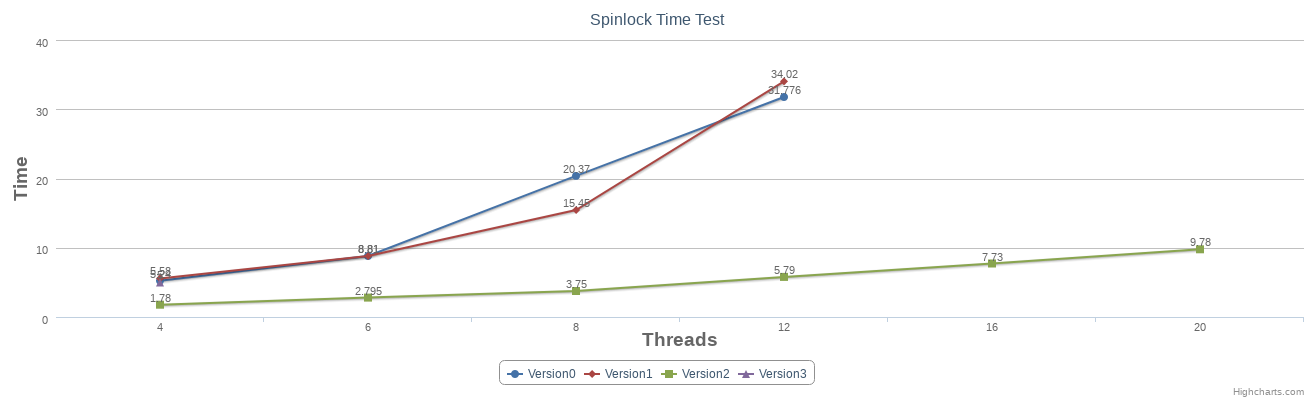
\includegraphics[width=400px,height = 110px]{0.png}}
		\end{center}
		It's basically accorded with our assumptions. But the TICKET spinlock performs much worse than our expectations. Why? Trying to be fair is good but fairness isn't always coming with efficiency. It does perform better than the \emph{version0} and \emph{version1} because the cpu'c cores' number fits with the thread  number. But when there exists a cpu resource race, it performs really worse then \emph{version0} and \emph{version1}.  Let's focus on the threads racing in a cpu core. Assuming that 5 threads are competing for cpu core. Thread1 asks for a number 1, Thread2 asks for a number 2..etc. Assuming that now it's thread1' turn, but it's not in the core,(Maybe the costumer 1 goes to the toilet...) the cpu can go on the process when it goes back, it really takes a long time. We improve the fairness to improve the efficiency. But they're not in a linear relationship. 
	\end{itemize}
	\subsection{Add Ons}
	 I'm not satisfied with the \texttt{version3}'s performance, so I retry again in a more sophisticated way called \texttt{queue\_control\_lock}. It comes with more memory consumption, but performs as well as the best spinlock. \\
	 \subsubsection{A concurrent queue}
	 It's a really tricky queue implementation. To finish it, we should define some queue conditions.\\
	 \begin{itemize}
	 	\item \textbf{empty} : When the queue's head meet with queue's tail, empty. \\
	 	\item \textbf{dequeue} : Who gets permission is the one who changes the head to head->next. We need an atomic operation to safely change the head to the next. And we the element leaves, it should be set to zero to signify that it has gone.\\
	 	\item \textbf{enqueue} : A new node comes with value set to 1(\texttt{in queue mark}) and next set to NULL. Who gets the permission to the tail is the one who changes the tail->next to the new node. Then we should change the tail to tail->next. But this time, the thread doesn't have to make sure that it has successfully changed the tail because  it's the only one who can changes the tail because it's the only on in the code section which changes the tail.
	 \end{itemize}
 	\begin{lstlisting}
void queue_init(lqueue_t *q)
{
	lnode_t *tmp = (lnode_t*)malloc(sizeof(lnode_t));
	tmp->value = 0; tmp->next = NULL;
	q->head = tmp;  q->tail = tmp;
}
void queue_enqueue(lqueue_t *q,int * val)
{
	lnode_t *tmp = (lnode_t*)malloc(sizeof(lnode_t));
	tmp->value = val;
	tmp->next = NULL;
	lnode_t *r;
	do
	{
		r = q->tail;
	}while(!__sync_bool_compare_and_swap(&(r->next),NULL, tmp));
	__sync_bool_compare_and_swap(&(q->tail),r,tmp);
}
int* queue_dequeue(lqueue_t *q)
{
	lnode_t* p;
	do
	{
		p = q->head;
	}while(!__sync_bool_compare_and_swap(&(q->head),p,p->next));
	*(p->next->value) = 0;
	return p->next->value;
}
int queue_empty(lqueue_t *q)
{
	if(q==NULL || q->head==q->tail )
		return 1;
	return 0;
}
 	\end{lstlisting}
	\subsubsection{Lock}
		A guard is set to ensure everyone comes to the code set is mutual exclusive. But after futex-sleep, the code section is not guarded. So we need a new flag to ensure it, so we reuse the flag to guard the critical zone. After performance test, the efficiency is close to the fastest spinlock. \\
	\begin{lstlisting}
void spinlock_init(spinlock_t* inLock)
{
	inLock->flag = 0;
	inLock->guard = 0;
	inLock->q = (lqueue_t *)malloc(sizeof(lqueue_t));
	queue_init(inLock->q);
}
void spinlock_acquire(spinlock_t* inLock)
{
	while(xchg(&inLock->guard,1) == 1);
	if(__sync_bool_compare_and_swap(&inLock->flag,0,1))
	{
		inLock->guard = 0;
	}
	else
	{
		int *tmp = (int*)malloc(sizeof(int));
		*tmp = 1;
		queue_enqueue(inLock->q,tmp);
		inLock->guard = 0;
		while(!__sync_bool_compare_and_swap(
					&inLock->flag,0,1))
		{
			futex_wait(tmp, 1);
		}
	}
}
void spinlock_release(spinlock_t* inLock)
{
	while(xchg(&inLock->guard,1) == 1);
	if(!queue_empty(inLock->q))
	{
		int *tmp = queue_dequeue(inLock->q);
	futex_post(tmp);
	}
	xchg(&inLock->flag,0);
	inLock->guard = 0;
}
	\end{lstlisting}
	\section{mutex Lock}
		When we need a public resource for a relatively long time, it's too wasted for a thread to keep asking for the critical zone continuously. So we can let it sleep until the other thread releases it. To accomplish it, we need a system function called futex which can be used to awake and sleep the thread. 
		\subsection{Implementation}
		\subsubsection{\textbf{version1.0}}
		It's a version that is completely derived from the mutex idea without any optimization. When a thread comes to visit the mutex lock, if it's not locked, the thread just locks it. Else, futex\_wait and waits for others to awake it. Here's the lock's Finite State Machine. \\
		\begin{center}
			\makebox[\textwidth]{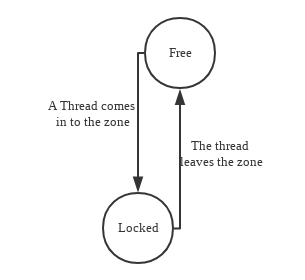
\includegraphics[width=200px,height = 200px]{4.png}}
		\end{center}
		And here's the code: \\
		\begin{lstlisting}
#define UNLOCKED 0
#define LOCKED   1
void mutex_acuire(mutex_t* mutex)
{
	while(__sync_val_test_and_set(mutex,LOCKED))
		futex_wait(mutex,COMPETE);
}
void mutex_release(mutex_t *mutex)
{
	*mutex = UNLOCKED;
}
		\end{lstlisting}
		\subsubsection{\textbf{version1.1}}
		There're only two phases in the \emph{version1.0}, so it's a natural idea to add a new phase before sleeping to improve performance by avoiding some occasions like in 2 threads' race, if both of them get in and get out quickly, it's a heavy burden for system to frequently be trapped into the sleep state and awake the sleep threads again and again. And in my implementation, I divided 3 phases called \textit{UNLOCKED}, \textit{LOCKED}, \textit{COMPETE}. \\
		\begin{itemize}
			\item \textit{UNLOCKED} \\
				No one is in the critical zone or a thread just leaves it but no one has asked for the lock. \\
			\item \textit{LOCKED} \\
				A new thread gets into the thread and the lock is free, then before it gets into the critical zone, it lifts the lock to 1 first. \\
			\item \textit{COMPETE} \\
				Now the lock is visited twice without being set UNLOCKED, it tells every thread it's in the \textit{COMPETE} state. Now if someone is asking for the lock, it's just trapped into sleep mode. \\
		\end{itemize}
		Here's the finite state machine: \\
		\begin{center}
			\makebox[\textwidth]{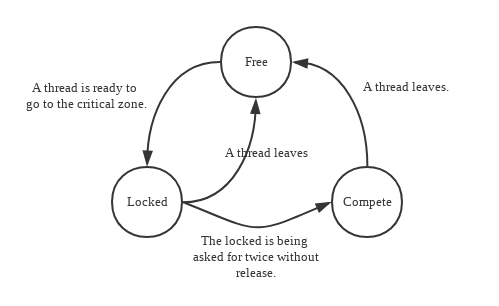
\includegraphics[width=350px,height = 200px]{6.png}}
		\end{center}
		And here's the code: \\
		\begin{lstlisting}
void mutex_acquire (mutex_t* mutex)
{
	//check if mutex is zero, if it is, unlocked to locked
	//state==2 means that it's congesting now state == 1 
	//means that it will be locked in next visit
	int state = __sync_val_compare_and_swap(mutex,
		UNLOCKED,LOCKED);
	//if not locked 
	while(state)
	{
		//if it is now congested or locked
		if(state == COMPETE || __sync_val_compare_and_swap(
		                            mutex, LOCKED, COMPETE))
			futex_wait(mutex,COMPETE);
		state = __sync_lock_test_and_set(mutex, LOCKED);
}
		\end{lstlisting}
		\subsubsection{\textbf{version1.2}}
		Now there's a choice that we should pay our attention on is that a thread just being awakened should goto which kind of state, \textit{UNLOCKED} or \textit{COMPETE}? Both seem plausible, so we need some experiments. \\
		\subsubsection{\textit{version2.0}}
		It's the version implemented in the old \emph{glibc}. The idea of it is that the top bit is used to signify the mutex state(\textit{UNLOCKED}, \textit{LOCKED}) and the value is used to tell its ID. But in my implementation, it performs worse than \emph{version1.0}. It's because that some \textit{futex\_post(s)} may be lost to awake a sleeping thread and the bitset operation is an enormous expense.\\
		Here's the code. \\
		\begin{lstlisting}
void mutex_acquire (mutex_t* mutex)
{
	if (atomic_bit_test_set (mutex,31)==0)
		 return;
	atomic_increment(mutex);
	int v;
	while(atomic_bit_test_set (mutex,31)!=0)
	{
		v = *mutex;
		if( v >= 0 ) continue;
		futex_wait (mutex,v);
	}
	atomic_decrement (mutex);
	return;
}
		\end{lstlisting}  
		\subsection{Performance}
		Here's the comparison, from which we can clearly say that the \textbf{version1.2} is a winner. \\
		\begin{center}
			\makebox[\textwidth]{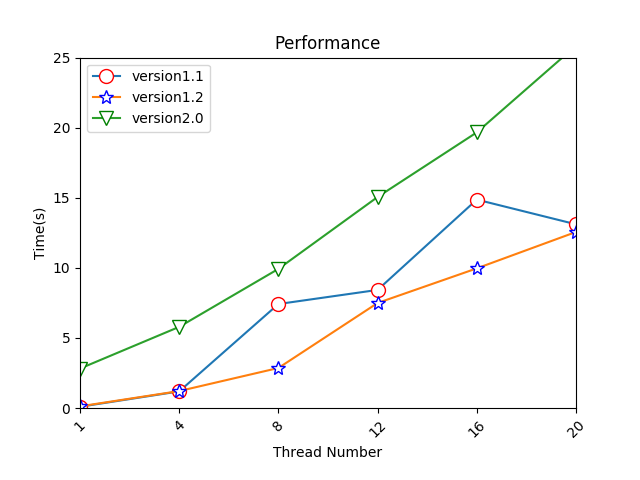
\includegraphics[width=350px,height = 200px]{5.png}}
		\end{center}
	\section{Tow phase Lock}
		Actually, the \textit{version1.1} and \textit{version1.2} is a combination of spinlock and mutex lock. But to adjust the parameter is essential to improve the performance, so we need to complete our code. Here's a simple implementation. \\
		\begin{lstlisting}
void twophase_acquire(twophase_t *mylock)
{
	int state = __sync_val_compare_and_swap(
				mylock,UNLOCKED,LOCKED);
    while(state)
	{
		if(state == COMPETE || __sync_val_compare_and_swap(
						mylock, LOCKED, COMPETE))
			futex_wait(mylock,COMPETE);
		for(int j=0;j<10;j++)
		{
			state = __sync_val_compare_and_swap(mylock, 
						UNLOCKED, COMPETE);
			if(!state)return;
		}
	}
}
void twophase_release(twophase_t *mylock)
{
	if( __sync_lock_test_and_set(mylock,0) == COMPETE)
		futex_post(mylock);
}
		\end{lstlisting}
		The comparison comes in after we finish our data structure.
	\section{Data Structure}
		\subsection{\textbf{Counter}}
		My version is simple, just count. (Approximate counter is scalable but not accurate)\\
		\subsection{\textbf{List}}
		The list is simple but where should we set the clock? Each element or the whole list? Assuming that we give every element a lock, then when we lookup the whole list, we need to acquire and release every element in the whole list as well as in the insert and delete operation which is unreasonable. So forget it, just give the whole list a lock. \\
		Here's the data structure but without function which is easy to understand and simple: \\
		\begin{lstlisting}
typedef struct list_value
{
	unsigned int	   key;
	struct list_value* next;
}list_value;

typedef struct list_t
{
	lock_t lck;
	list_value* root;
}list_t
		\end{lstlisting}
		\subsection{\textbf{Hash}}
		It maintained some buckets and every bucket is a \textit{list}, so insert, delete and lookup operations are just calling the list function I implement before in the specific bucket. To be scalable, using a point to maintain memory instead of an array. Here's the data structure and \textit{init} function: \\
		\begin{lstlisting}
typedef struct hash_t
{
	int size;
	list_t *bucket;
}hash_t
void hash_init(hash_t *hash, int size)
{
	hash->bucket = (list_t*)malloc(sizeof(list_t)*size);
	hash->size=size;
	int i=0;
	for(;i<size;i++)
	{
		list_init(&(hash->bucket[i]));
	}
}

		\end{lstlisting}
	\section{Performance}
		\subsection{\textbf{in counter}}
		\begin{center}
			\makebox[\textwidth]{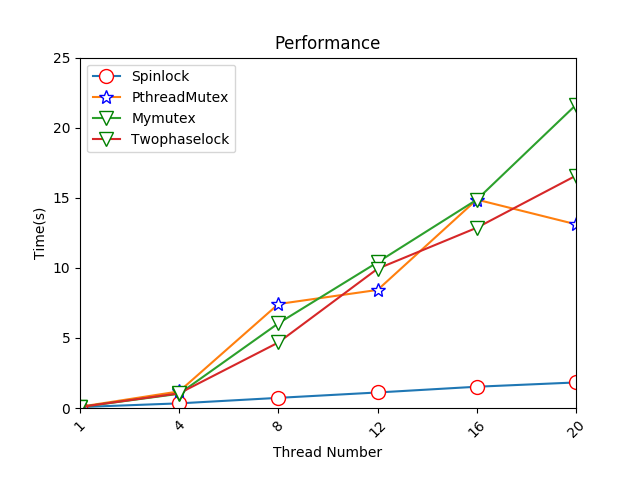
\includegraphics[width=350px,height = 200px]{1.png}}
		\end{center}
		\subsection{\textbf{in list}}
		\begin{center}
			\makebox[\textwidth]{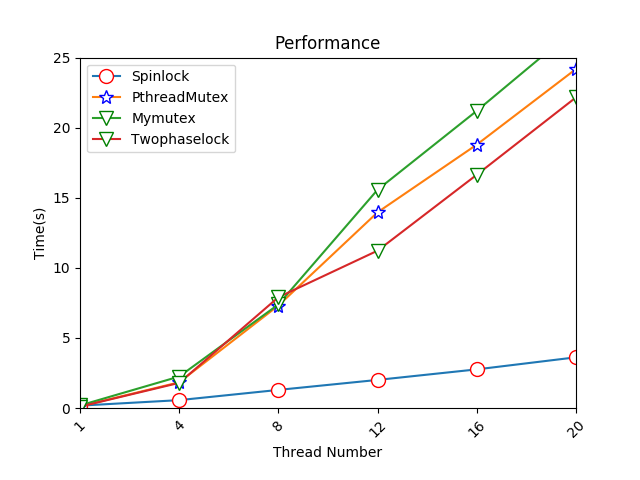
\includegraphics[width=350px,height = 200px]{2.png}}
		\end{center}
		\subsection{\textbf{in hash}}
		\begin{center}
			\makebox[\textwidth]{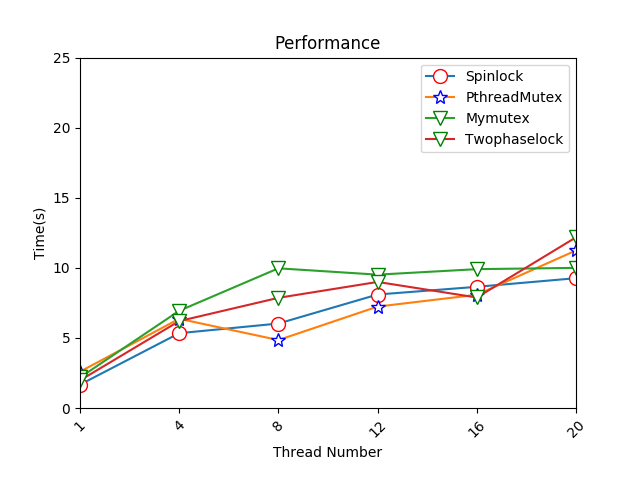
\includegraphics[width=350px,height = 200px]{3.png}}
		\end{center}
		From the diagram, we can clearly see that in the counter and list function, spinlock performed far better then mutex whatever how they were implemented. But in hash table, pthread mutex performes better. Spinlock is really powerful, then why actually we mutex is used wider then spinlock? It's because a well-implemented parallel program is visiting implementing critical zone as less  possible. So a program like increasing a counter 1e6 doing nothing else in each thread is meaningless, so after several asking, just sleep the thread is much better then keeping asking. It's not only about the cpu's computing resource's waste but also the bus bottleneck. When a cpu keeps asking for bus control, it sometimes blocks other cpu's visit. 
\end{document}

